\documentclass[10pt,a4paper]{article}
\usepackage[utf8]{inputenc}
\usepackage{amsmath}
\usepackage{amsfonts}
\usepackage{amssymb}
\usepackage{makeidx}
\usepackage{graphicx}
\usepackage[left=2cm,right=2cm,top=2cm,bottom=2cm]{geometry}
\author{\textbf{Universidad Politécnica De La Zona Metroplitana de Guadalajara }\\\\ \textbf{Alumno:}\\ Jiménez Cortés Raúl \\\\ \textbf{Carrera:}\\ Ingeniería Mecatrónica\\\\ \textbf{Grado Y Grupo:}\\ 4ª "B" \\\\
\textbf{Materia:}\\ Sistemas Electrónicos De Interfaz \\\\ \textbf{Profesor:}\\ Morán Garabito Carlos Enrique}
\title{\textbf{EV-2-2-EXPLICAR LOS ARREGLOS Y PARÁMETROS DE LOS AMPLIFICADORES CLASE A}}
\date{\textbf{01/Octubre/2019}}


\begin{document}
\begin{figure}
\centering

\includegraphics[scale=1]{Pa.jpg}
\end{figure}

\maketitle

\newpage
\section{Apmlificador Clase A}
Son aquellos amplificador cuyas etapas de potencia consumen corrientes altas y continuas de su fuente de alimentación, independientemente de si existe señal de audio o no.
Cuando una señal de entrada a un circuito presenta un voltaje de amplitud suficiente, las etapas conectadas a continuación han de entregar ganancia de corriente para que de esta forma, poder excitar convenientemente a la carga. Estas estapas se llaman comunmente amplificadores de potencia o etapas de potencia y se dividen basicamente en cuatro grupos o clases: A, B, AB y C, dependiendo de la forma de l aseñal de salida a partir de una entrada señoidal.\\
un ampliificador clase A ofrece una señal de salida igual a la de entrada, pero amplificada. en clase B solo un semiciclo y en clase C parte de un semiciclo de dicha señal (imagen 1). \\
\begin{figure}[hbtp]
\centering
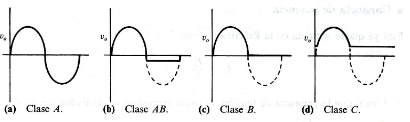
\includegraphics[scale=1]{clase.png}
\caption{Salidas De Los Amplificadores De Potencia.}
\end{figure}\\\\
\textbf{Características}\\
Esta amplificación presenta el inconveniente de generar una fuerte y constante emisión de calor. No obstante, los transistores de salida están siempre a una temperatura fija y sin alteraciones.\\
En general, se afirma que esta clase de amplificación es frecuente en circuitos de audio y en los equipos domésticos de gama alta, ya que proporcionan una calidad de sonido potente y de muy buena calidad.\\
Los amplificador de clase A a menudo consisten en un transistor de salida conectado al positivo de la fuente de alimentación y un transistor de corriente constante conectado de la salida al negativo de la fuente de alimentación.\\
La señal del transistor de salida modula tanto el voltaje como la corriente de salida. Cuando no hay señal de entrada, la corriente de polarización constante fluye directamente del positivo de la fuente de alimentación al negativo, resultando que no hay corriente de salida, se gasta mucha corriente. Algunos amplificador de clase A más sofisticados tienen dos transistores de salida en configuración push-pull.\\\\\\
\textbf{Ventajas}\\
La clase A se refiere a una etapa de salida con una corriente de polarización mayor que la máxima corriente de salida que dan, de tal forma que los transistores de salida siempre están consumiendo corriente. La gran ventaja de la clase A es que es casi lineal, y en consecuencia la distorsión es menor.\\\\\\
\textbf{Deventajas}\\
La gran desventaja de la clase A es que es poco eficiente, se requiere un amplificador de clase A muy grande para dar 50 W, y ese amplificador usa mucha corriente y se pone a muy alta temperatura. 
\newpage
Los amplificadores emisores comunes son el tipo de amplificador más comúnmente usado, ya que pueden tener una ganancia de voltaje muy grande.\\
Los amplificadores Common Emitter (CE) están diseñados para producir una gran oscilación de voltaje de salida desde un voltaje de señal de entrada relativamente pequeño de solo unos pocos milivoltios y se usan principalmente como "amplificadores de pequeña señal".\\\\

\begin{center}
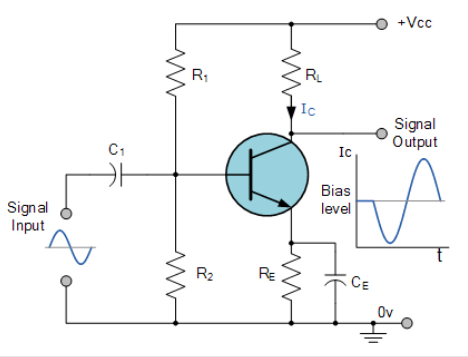
\includegraphics[scale=0.5]{img.png}\\\
\end{center}
Sin embargo, algunas veces se requiere un amplificador para manejar grandes cargas resistivas como un altavoz o para conducir un motor en un robot y para este tipo de aplicaciones donde se necesitan altas corrientes de conmutación. Se requieren amplificadores de potencia.\\
La función principal del amplificador de potencia, que también se conoce como "amplificador de señal grande", es suministrar potencia, que es el producto del voltaje y la corriente de la carga. Básicamente, un amplificador de potencia también es un amplificador de tensión, con la diferencia de que la resistencia de carga conectada a la salida es relativamente baja, por ejemplo, un altavoz de 4 ohm o 8 ohm resulta en corrientes altas que fluyen a través del colector del transistor.\\
Debido a estas altas corrientes de carga, los transistores de salida utilizados para las etapas de salida del amplificador de potencia, como el 2N3055, necesitan tener mayores niveles de tensión y potencia que los generales utilizados para amplificadores de señal pequeña como el BC107.\\
Para entregar la máxima potencia de CA a la carga, mientras consumimos la mínima potencia de CC posible del suministro, nos preocupa principalmente la (eficiencia de conversión) del amplificador.\\
Sin embargo, una de las principales desventajas de los amplificadores de potencia y especialmente del amplificador de Clase A es que su eficiencia de conversión general es muy baja ya que las grandes corrientes significan que se pierde una cantidad considerable de energía en forma de calor. La eficiencia porcentual en los amplificadores se define como la potencia de salida rms disipada en la carga dividida por la potencia total de CC tomada de la fuente de suministro como se muestra a continuación.\\
\textbf{Eficiencia Del Amplificador De Potencia}\\
\begin{center}
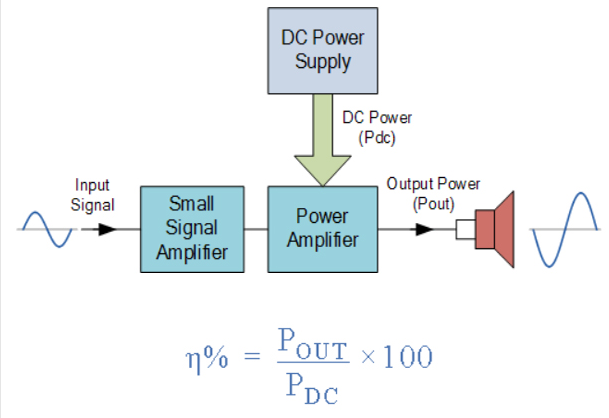
\includegraphics[scale=0.3]{img1.png} 
\end{center}
Dónde:
n- es la eficiencia del amplificador.
Pout - es la potencia de salida de los amplificadores entregada a la carga.
Pdc - es la potencia de CC tomada del suministro.
Para un amplificador de potencia, es muy importante que la fuente de alimentación de los amplificadores esté bien diseñada para proporcionar la máxima potencia continua disponible a la señal de salida.\\
\newpage
El amplificador de Clase A es la forma más simple de amplificador de potencia que utiliza un solo transistor de conmutación en la configuración de circuito de emisor común estándar como se ha visto anteriormente para producir una salida invertida. El transistor siempre está polarizado en "ON" para que conduzca durante un ciclo completo de la forma de onda de la señal de entrada, produciendo la mínima distorsión y la máxima amplitud de la señal de salida.\\
Esto significa que la configuración del amplificador de clase A es el modo de funcionamiento ideal, ya que no puede haber distorsión de cruce o desconexión a la forma de onda de salida incluso durante la mitad negativa del ciclo. Las etapas de salida del amplificador de potencia de Clase A pueden usar un único transistor de potencia o pares de transistores conectados entre sí para compartir la corriente de alta carga. Considere el circuito amplificador Clase A a continuación.\\
\textbf{Circuito Amplificador De Una Sola Etapa}\\
\begin{center}
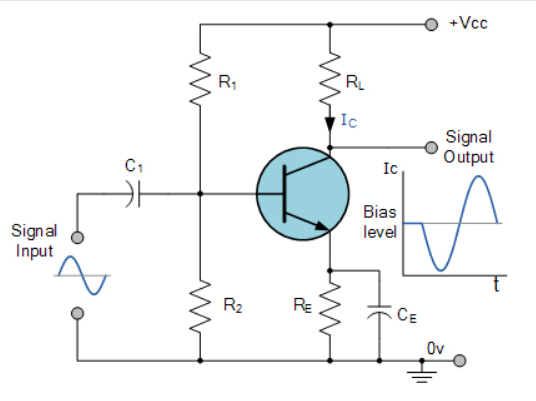
\includegraphics[scale=0.4]{img2.png} 
\end{center}

Utiliza un transistor de extremo único para su etapa de salida con la carga resistiva conectada directamente al terminal colector. Cuando el transistor se "enciende", se hunde la corriente de salida a través del Colector, lo que resulta en una caída de voltaje inevitable a través de la resistencia del Emisor, limitando así la capacidad de salida negativa.\\
La eficiencia de este tipo de circuito es muy baja (menos del 30 porciento) y ofrece pequeñas salidas de potencia para un gran drenaje en la fuente de alimentación de CC. Una etapa de amplificador de Clase A pasa la misma corriente de carga incluso cuando no se aplica señal de entrada, por lo que se necesitan disipadores de calor grandes para los transistores de salida.\\
Sin embargo, otra forma simple de aumentar la capacidad de manejo actual del circuito mientras que al mismo tiempo se obtiene una mayor ganancia de potencia es reemplazar el transistor de salida simple con un transistor Darlington . Estos tipos de dispositivos son básicamente dos transistores dentro de un solo paquete, un pequeño transistor "piloto" y otro transistor de "conmutación" más grande. La gran ventaja de estos dispositivos es que la impedancia de entrada es adecuadamente grande, mientras que la impedancia de salida es relativamente baja, reduciendo así la pérdida de potencia y, por lo tanto, el calor dentro del dispositivo de conmutación.\\
\textbf{Configuraciones del transistor Darlington}\\
\begin{center}
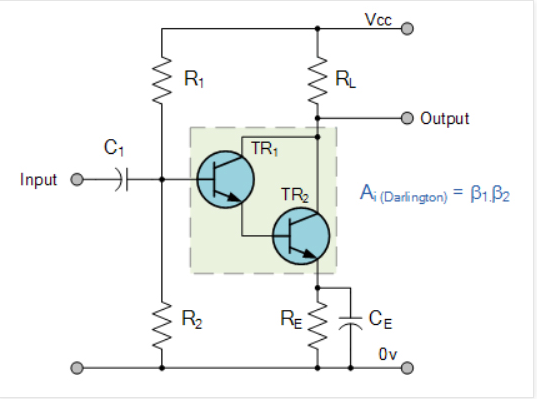
\includegraphics[scale=0.4]{img3.png} 
\end{center}
La ganancia de corriente total Beta (B) o el valor de hfe de un dispositivo Darlington es el producto de las dos ganancias individuales de los transistores multiplicadas juntas y valores de B muy elevados junto con altas corrientes de colector son posibles en comparación con un solo circuito de transistor.\\
Para mejorar la eficiencia total de potencia del amplificador de Clase A , es posible diseñar el circuito con un transformador conectado directamente en el circuito colector para formar un circuito llamado amplificador acoplado a transformador . El transformador mejora la eficiencia del amplificador al hacer coincidir la impedancia de la carga con la de la salida de los amplificadores usando la relación de vueltas ( n ) del transformador y un ejemplo de esto se da a continuación.\\
\textbf{Circuito amplificador acoplado a transformador}\\
\begin{center}
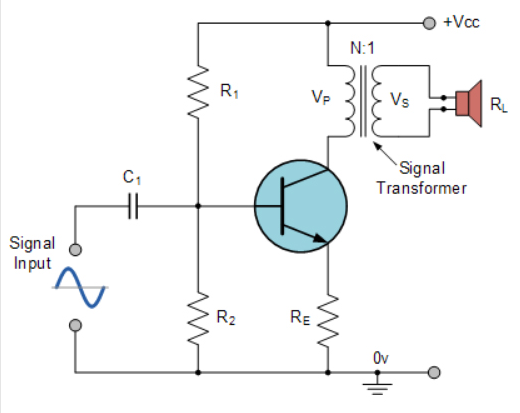
\includegraphics[scale=0.4]{img4.png} 
\end{center}
Como la corriente del colector, Ic se reduce por debajo del punto Q quieto establecido por la tensión de polarización básica, debido a las variaciones en la corriente base, el flujo magnético en el núcleo del transformador se colapsa causando una fem inducida en los devanados primarios del transformador. Esto hace que una tensión instantánea del colector aumente a un valor del doble de la tensión de alimentación de 2 Vcc, lo que da una corriente de colector máxima de dos veces Ic cuando el voltaje del colector está en su mínimo. Entonces la eficiencia de este tipo de configuración del amplificador de clase A se puede calcular de la siguiente manera.\\
El voltaje del colector de rms se da como:\\
\begin{center}
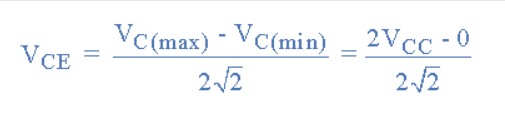
\includegraphics[scale=0.3]{img5.png} 
\end{center}
La corriente del recopilador rms se da como:\\
\begin{center}
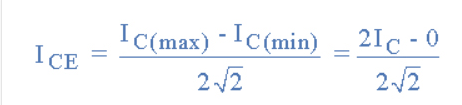
\includegraphics[scale=0.3]{img6.png} 
\end{center}
La potencia rms entregada a la carga (Pac) se da por lo tanto como sigue:\\
\begin{center}
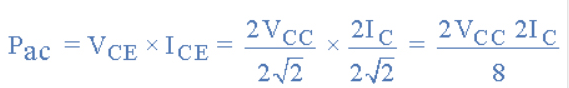
\includegraphics[scale=0.4]{img7.png} 
\end{center}
La potencia promedio extraída del suministro (Pdc) viene dada por:\\
\begin{center}

\includegraphics[scale=0.4]{img8.png} 
\end{center}
y, por lo tanto, la eficacia de un amplificador Clase A acoplado a transformador se da como:\\
\begin{center}
 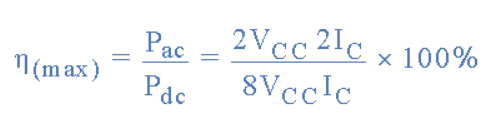
\includegraphics[scale=0.4]{img9.png} 
 \end{center} Un transformador de salida mejora la eficiencia del amplificador al hacer coincidir la impedancia de la carga con la de la impedancia de salida del amplificador. Al utilizar un transformador de salida o de señal con una relación de espiras adecuada, las eficiencias del amplificador de clase A que alcanzan el 40 porciento son posibles con la mayoría de los amplificadores de potencia de clase A disponibles en este tipo de configuración.\\
Sin embargo, el transformador es un dispositivo inductivo debido a sus bobinados y núcleo, por lo que es mejor evitar el uso de componentes inductivos en los circuitos de conmutación del amplificador, ya que cualquier fuerza electromagnética generada puede dañar el transistor sin la protección adecuada.\\
También otra gran desventaja de este tipo de circuito amplificador de clase A acoplado a transformador es el costo adicional y el tamaño del transformador de audio requerido.\\
El tipo de "Clase" o clasificación que se le da a un amplificador realmente depende del ángulo de conducción, la porción de 360 o del ciclo de la forma de onda de entrada, en el cual el transistor está conduciendo. En el amplificador de Clase A el ángulo de conducción es un completo 360 o o 100 porciento de la señal de entrada, mientras que en otras clases de amplificadores el transistor conduce durante un ángulo de conducción menor.\\
Es posible obtener una mayor potencia de salida y eficiencia que la del amplificador de clase A mediante el uso de dos transistores complementarios en la etapa de salida con un transistor de tipo NPN o N-channel, mientras que el otro transistor es un PNP o P-channel (el complemento) tipo conectado en lo que se llama una configuración "push-pull".


\bibliography{Tarea3}{http://tutorialesdeelectronicabasica.blogspot.com/2018/06/el-amplificador-de-clase-es-un.html}
\bibliographystyle{plain}
\end{document}